\section{Motivating Examples}

As a first motivating example, imagine a user was to reconstruct the filter that was used to transform an audio clip.
In this case the user has the original audio file, and the transformed audio file, but does not know how this transformation happened.
In the standard approach, a user would need to be a domain expert and listen to the two files, and aurally estimate which kinds of filters were used to achieve the transformation.
Once the user has some suspicion as to the appropriate filter types that will be needed, the user must write a program in some language (SuperCollider, MaxMSP, CSound, etc) that implements the DSP filter the user has in mind.
Further still, the user will then need to spend time tweaking the filter parameters to find the best fit.

In contrast, with DSP-PBE, the user simply provides our tool with the original audio, and the transformed audio, and will automatically receive a DSP filter that approximates the transformation.
This was the approach used for the audio files in Figure~\ref{fig:test}.
In this example, a user provided a clip of a 'cartoon spring' in Figure~\ref{fig:inEx}, and the same sound as it had been transformed with a low-pass filter at 800 Hz, $lpf(800)$, as shown in Figure~\ref{fig:outEx}.
However the nature of the transformation is unknown to the user and they wish to discover the filter needed.
Our DSP-PBE tool is able to synthesize a filter $lpf(947)$, that when applied to the original sound, produces the waveform shown in Figure~\ref{fig:synthEx}.
While the solution is not exact, the difference is not significantly noticeable to an untrained ear.

\begin{figure}
\centering
\begin{subfigure}{.32\linewidth}
  \centering
  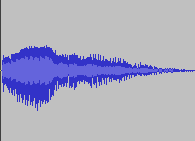
\includegraphics[width=.9\textwidth]{figs/original.png}
  \caption{Input example}
  \label{fig:inEx}
\end{subfigure}%
\begin{subfigure}{.32\linewidth}
  \centering
  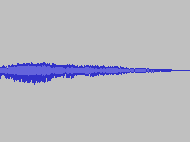
\includegraphics[width=.9\textwidth]{figs/lpf800.png}
  \caption{Output example}
  \label{fig:outEx}
\end{subfigure}
\begin{subfigure}{.32\linewidth}
  \centering
  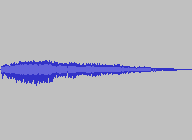
\includegraphics[width=.9\textwidth]{figs/lpf950.png}
  \caption{Generated}
  \label{fig:synthEx}
\end{subfigure}
\caption{The waveforms (a) and (b) are provided as examples, and DSP-PBE synthesizes a filter that produces (c).}
\label{fig:test}
\end{figure}

More creative applications?
